\documentclass{standalone}
\usepackage[utf8]{inputenc}
\usepackage{xcolor}
\usepackage{tikz}
\usepackage{kpfonts}

\usetikzlibrary{arrows}

\begin{document}
\pagestyle{empty}

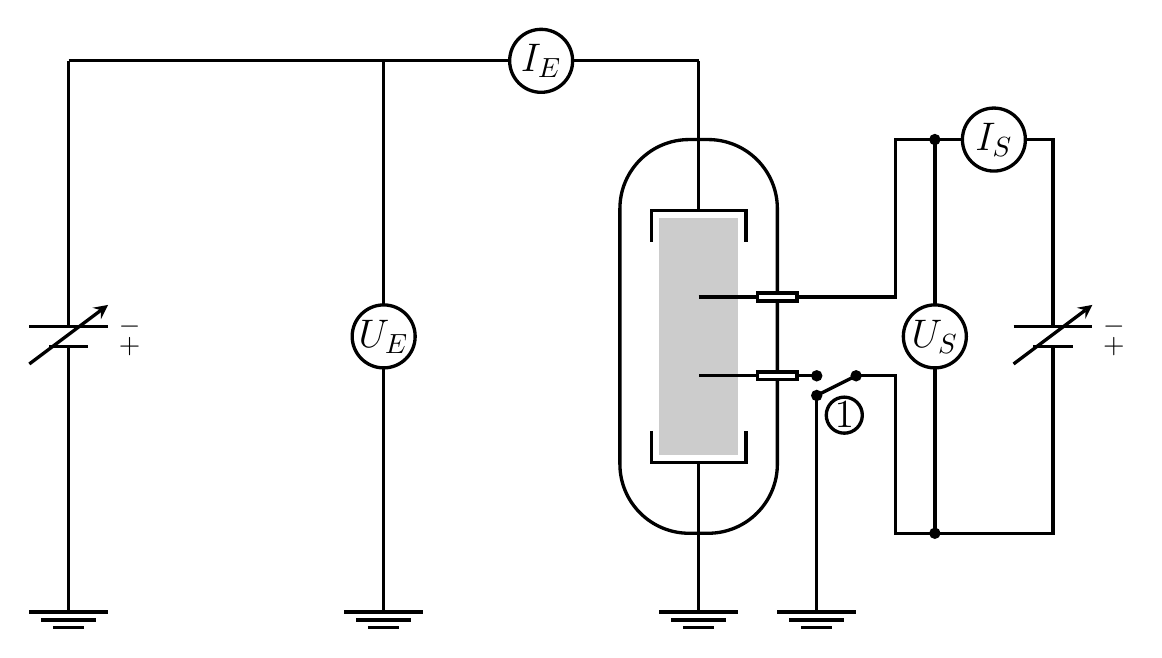
\begin{tikzpicture}[scale=1]

	\tikzset{every path/.style={line width=1.2pt}}

	\tikzset{>=stealth}
	
	%\draw (0,0) grid (14,7);

	%Erdungen
	\foreach \x in {1,5,9} {
		\draw (\x,0) -- (\x + 1,0);
		\draw (\x+0.15,-0.1) -- (\x + 0.85,-0.1);
		\draw (\x+0.3,-0.2) -- (\x + 0.7,-0.2);
		\draw (\x+.5,0) -- (\x+.5,7);
	}
	\draw (1.5,7) -- (9.5,7);
	
	%Tube
	\draw[rounded corners=25] (8.5,1) rectangle (10.5,6);
	
	\filldraw[fill=white] (8.9,2.3) -- (8.9,1.9) -- (10.1,1.9) -- (10.1,2.3);
	
	\filldraw[fill=white] (8.9,4.7) -- (8.9,5.1) -- (10.1,5.1) -- (10.1,4.7);
	
	\fill[black!20] (9,2) rectangle (10,5);
	
	%Sonden
	\draw (9.5,4) -- (12,4) -- (12,6) -- (14,6) -- (14,1) -- (12,1) -- (12,3)-- (9.5,3);
	\draw (12.5,6) -- (12.5,1); \filldraw (12.5,6) circle (0.05); \filldraw (12.5,1) circle (0.05);
	\foreach \x in {0,1} {
		\filldraw[fill=white] (10.25,2.95 + \x) rectangle (10.75,3.05 + \x);
	}
	
	%Spannungserzeugung
	\foreach \x in {0,12.5} {
		\fill[white] (1 + \x,3.375) rectangle (2 + \x,3.625);
		\draw (1 + \x,3.625) -- (2 + \x, 3.625) node [right] {$-$};
		\draw (1.25 + \x,3.375) -- (1.75 + \x, 3.375) node [right, pos=1.5] {$+$};
		\draw[->] (1 + \x,3.15) -- (2 + \x,3.9);
		%\draw[->, bend left] (2.5 + \x,4.25) to[out=30,in=150] (2.5 + \x,2.75);
	}
	
	%Messgeräte
	\filldraw[fill=white] (5.5, 3.5) circle (0.4) node  {\Large $U_{\text{\scriptsize E}}$};
	\filldraw[fill=white] (12.5, 3.5) circle (0.4) node {\Large $U_{\text{\scriptsize S}}$};
	\filldraw[fill=white] (7.5, 7) circle (0.4) node {\Large $I_{\text{\scriptsize E}}$};	
	\filldraw[fill=white] (13.25, 6) circle (0.4) node {\Large $I_{\text{\scriptsize S}}$};
	
	%Alternative Schaltung
	\fill[white] (11,2.9) rectangle (11.5,3.1);
	\filldraw (11,3) circle (0.05);
	\filldraw (11.5,3) circle (0.05);
	\draw (11.5,3) -- (11,2.75);
	\draw (11.35,2.5) node [circle, inner sep = 0.5pt, draw] {\Large 1};
	\draw (11,2.75) -- (11,0);
	\filldraw (11,2.75) circle (0.05);
	\draw (10.5,0) -- (10.5 + 1,0);
	\draw (10.5+0.15,-0.1) -- (10.5 + 0.85,-0.1);
	\draw (10.5+0.3,-0.2) -- (10.5 + 0.7,-0.2);

\end{tikzpicture}

\end{document}